\chapter{MATERIALS AND METHODS - Yeast8}

\section{Consensus \emph{S. cerevisiae} Metabolic Model}
Variety of \emph{S. cerevisiae} genome-scale metabolic models have been used since 2003, and each reconstructed model introduced more manual curations, increasing gene numbers from annotations and better predictions regarding the previous ones \cite{lopes2017genome}. A consensus genome-scale metabolic model of \emph{S. cerevisiae}, Yeast8, is presented in an open-source, version-controlled maintainable way in 2019, claiming that the model can be represented and investigated in a systematic way using Git (https://git-scm.com/) and GitHub (https://github.com/) as a hosting service for the model repository \cite{lu2019consensus}. Systematic way of Yeast8 enables to study simultaneously in collaborative studies, provides record keeping of model changes, version updates, where each version of can be released periodically and accessible all the time (Figure \ref{fig:yeast8_github}).
\begin{figure}[ht]
\begin{center}
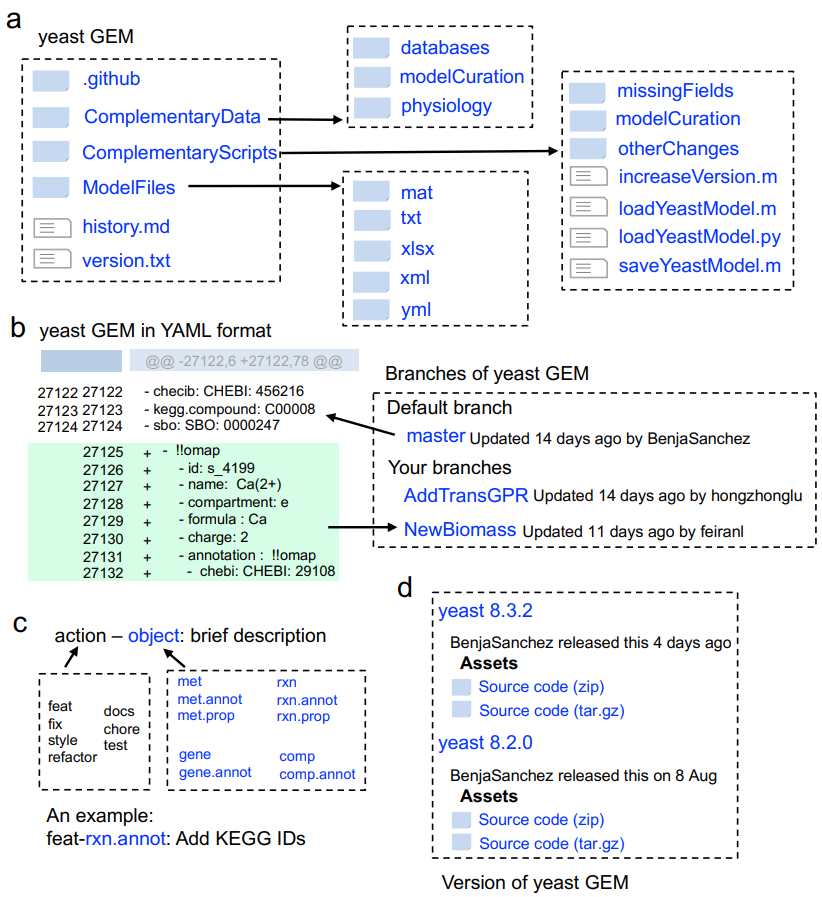
\includegraphics[width=0.9\columnwidth]{yeast8_github.png}
\end{center}
\caption[Repository of yeast GEM on GitHub]{Repository of yeast GEM on GitHub. Figure is taken from \cite{lu2019consensus}. ~ will be redrawned in thesis}
\label{fig:yeast8_github}
\end{figure}

Yeast8 model can be considered as an updated version of Yeast7 \cite{aung2013revising} with additional corrections based on the annotations available in KEGG and ChEBI, and several gene inclusions from the model iSce926 \cite{chowdhury2015using}. Final version of Yeast8, version 8.3.4 released on July 28, has 3991 reactions, 2691 metabolites, 1149 genes, 14 intracellular compartments.

All simulations in this chapter are done using Yeast8 v8.3.4 model which is hosted in Github (https://github.com/SysBioChalmers/yeast-GEM).

\section{Chemostat Simulation: GAM Fitting}
In order to make sure the \emph{in-silico} obtained growth rate predictions are in agreement with the physiological kinetic parameters obtained from real experiments, fine adjustment on the energy reactions is a requirement. Since the growth-associated maintenance (GAM) and non-growth associated maintenance (NGAM) energy reactions play a determinant role in simulations, fluxes through these reactions must be constrained to a fixed value. Flux of NGAM is constrained to 0.7 mmol gDWh\textsuperscript{-1} for aerobic, and 0 mmol gDWh\textsuperscript{-1} for anaerobic simulations as calculated in the previous studies \cite{nilsson2016metabolic}. For the estimatation of GAM, since it depends on the biomass composition, findings of a chemostat experiment \cite{van1998effect} is used as a guide to fit predictions to. Model is simulated iteratively with a range of values for GAM, and the best fit is found at the level of 55.25 mmol gDWh\textsuperscript{-1} (Figure \ref{fig:Gam_fitting}), GAM flux is constrained accordingly.

\begin{figure}
\begin{center}
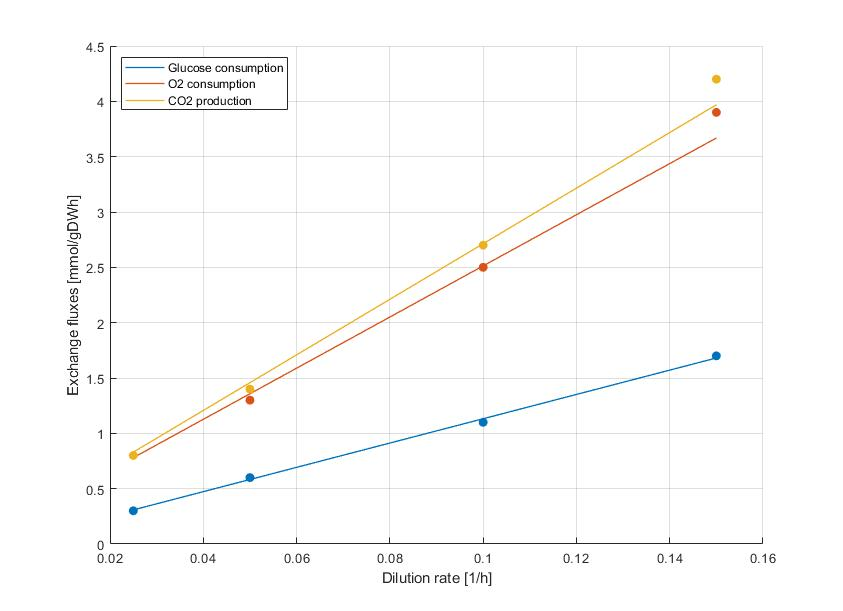
\includegraphics[width=0.8\columnwidth]{Gam_fitting.jpg}
\end{center}
\caption[Chemostat simulation to re-fit growth associated maintenance]{Chemostat simulation to re-fit growth associated maintenance.}
\label{fig:Gam_fitting}
\end{figure}


\section{Flux Balance Analysis}
Mathematical background of FBA...\hl{Review on "What is FBA?"}

In order to simulate batch conditions where minimal yeast medium is used, all the exchange reactions in the model are blocked first (lower bounds are set to 0). Then, only the exchange reactions of ions that are available to the cells in the experimental design (ammonium, phosphate, sulphate, iron(2+), H+, water, chloride, Mn\textsuperscript{2+}, Zn\textsuperscript{2+}, Mg\textsuperscript{2+}, sodium, Cu2\textsuperscript{2+}, Ca\textsuperscript{2+}, potassium) are set free (lower bounds are set to -1000). While oxygen and glucose uptake rates decreasing from 20 mmol gDWh\textsuperscript{-1} and increasing to 20 mmol gDWh\textsuperscript{-1}, respectively, fluxes on ethanol, acetate, glycerol, formate, succinate secretion reactions and growth rate is collected (Figure \ref{fig:fba}).
\hl{I need to show experimental results -preferably from the same article where I got expression data- on the figure to compare with my FBA results}


\begin{figure}
\begin{center}
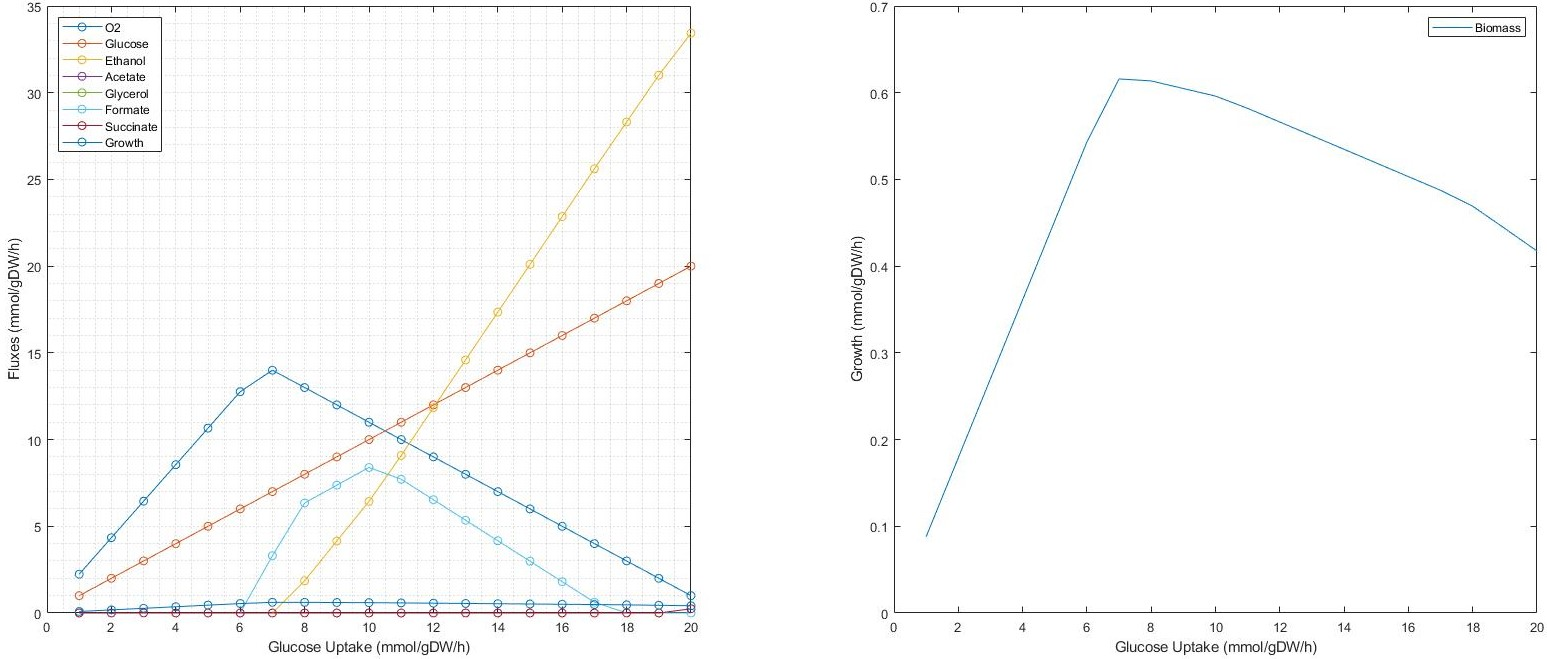
\includegraphics[width=1\columnwidth]{fba.jpg}
\end{center}
\caption[Flux balance simulation results]{Flux balance simulation results where oxygen uptake rate decreased and glucose uptake rate is increased simultaneously. Flux rates of several metabolites on the left, predicted growth rate on the right.}
\label{fig:fba}
\end{figure}


\section{Flux Variability Analysis}
Flux variability analysis (FVA) determines the minimum and maximum available fluxes for each reaction while obeying the provided constraints (for example fixed glucose uptake or growth rate). FVA is mainly used to evaluate the robustness of the model \cite{thiele2010functional}, to find alternative optimum states \cite{mahadevan2003effects}, to check flux distributions when growth is not at optimum level \cite{reed2004genome}, and in many other applications \cite{gudmundsson2010computationally}.


(Figure \ref{fig:fva})

\begin{figure}
\begin{center}
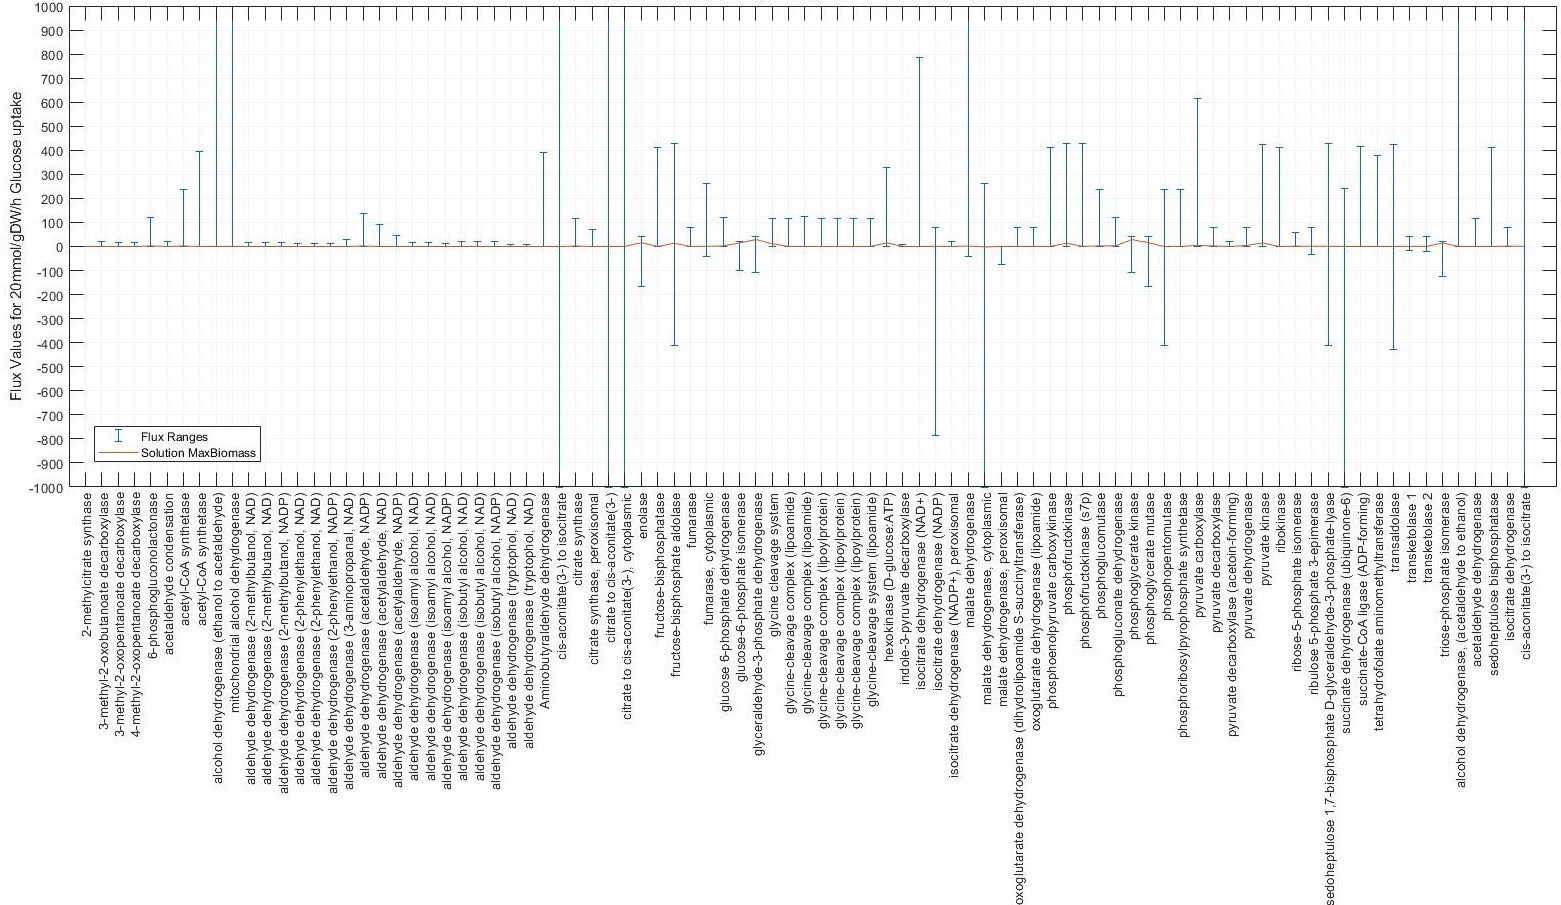
\includegraphics[width=1\columnwidth]{fva.jpg}
\end{center}
\caption[Minimum and maximum fluxes of Glycolysis, PPP and TCA reactions]{Minimum and maximum fluxes of Glycolysis, PPP and TCA reactions.}
\label{fig:fva}
\end{figure}

\section{Phenotype Phase Plane Construction}
\section{ACHRB Sampling}
\section{Expression Data Analysis}
\section{Integration of Expression Data Into Model}
